\section{Skillset and Toolset}

There is no clear market leader when it to the current tools available to incorporate AI into products and services.   
Toolsets have reached a relative level of maturity and stability almost to the commodity level, such that, once main operational concepts are grasped, toolsets present common features \cite{Landset2015} making skillsets transferable allowing for specific JCI R\&D units to leverage any currents licensing agreements to suit. All major cloud providers e.g. Amazon, Google and Microsoft bundle AI and ML into current products and services.  
Using such cloud providers and as a consequence transferring company data to external servers does raise issues beyond the scope of this text.  

Other notable tools are Matlab which contains a number of AI plugins although this is at best a prototyping tool, as it is not best known for deployment at scale.  

Programming languages popular with AI platforms are Python, Java, Scala and R. C++ is used to developed extensions to Python. Anecdotal evidence suggests that most interns (see "Pilot Scheme") are familiar with Python, which is emerging as a clear leader and number one choice for AI applications, notably Google Tensorflow makes use of Python as a primary programming language. Given the toolset is available on tap (pay-as-you-go cloud model), many of the tools are open-source and our intern population has the require skills, there is little additional investment required. Although there are concerns about open source tools, it is worth nothing that the US Defence Department is an investor in open source big data companies \cite{Defense2016} such as Cloudera Inc (NYSE: CLDR) proving that open source has come of age.

\begin{figure}[ht]
 \centering % avoid the use of \begin{center}...\end{center} and use \centering instead (more compact)
 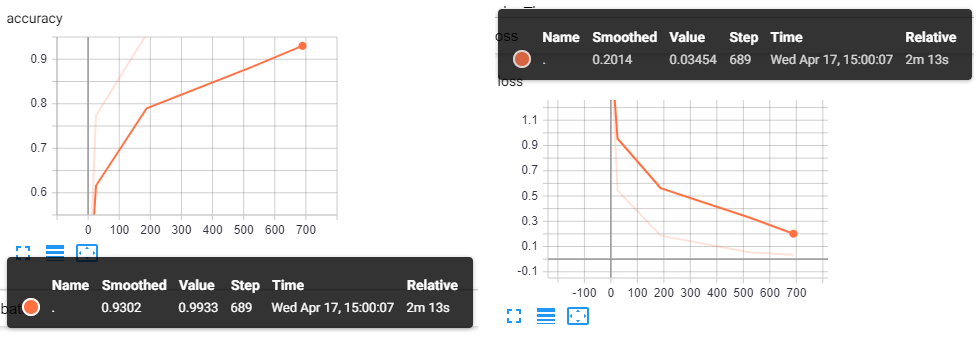
\includegraphics[width=140mm]{images/flowersdropout.png}
 \caption{Model accuracy and loss graphs on browser-based Google Cloud Tensorboard}
 \label{fig:sample}
\end{figure}

\begin{figure}[ht]
 \centering % avoid the use of \begin{center}...\end{center} and use \centering instead (more compact)
 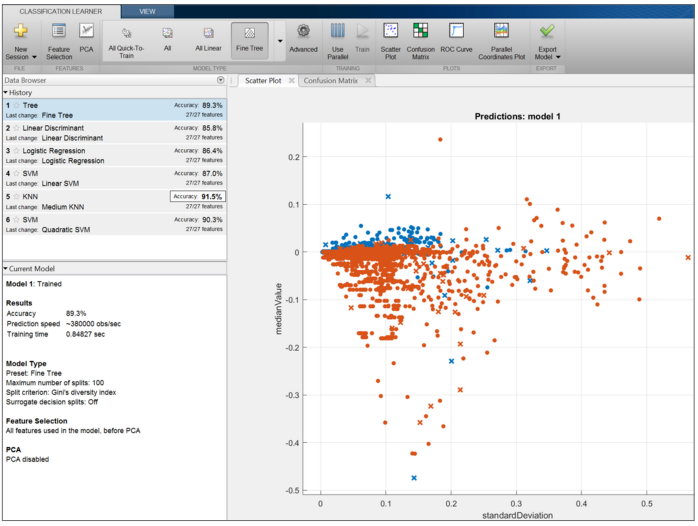
\includegraphics[width=140mm]{images/matlab-classification-learner.png}
 \caption{Model accuracy on Matlab's desktop based Classification Learner app}
 \label{fig:sample}
\end{figure}


